% !TeX root = ../../گزارش.tex
% !TeX encoding = UTF-8

در این پوشه به تمام مسیر‌های نرم‌افزار پرداخته شده است.
\begin{figure}[H]
	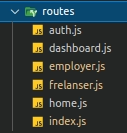
\includegraphics[width=.3\textwidth]{Folders-Files/routes/routes.png}
	\centering
	\caption{ساختار پوشه مسیر}
	\label{fig:folder:routes}
\end{figure}

\subsection{فایل index}
در این فایل مسیرهای برنامه تجمیع شده و تنها این فایل برای دسترسی به مسیرها فراخوانی می‌شود.
\begin{figure}[H]
	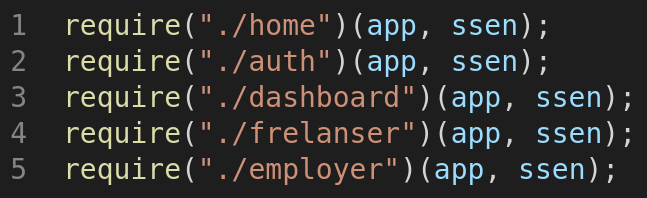
\includegraphics[width=.6\textwidth]{Folders-Files/routes/routes-index.png}
	\centering
	\caption{ساختار فایل index}
	\label{fig:file:routes:index}
\end{figure}
\paragraph{\lr{app}:}
شئ حاوی اطلاعات فریم‌ورک express.js است.
\paragraph{\lr{ssen}:}
شئ حاوی اطلاعات عمومی مانند اطلاعات کاربر، اطلاعات شاخه مسیرها و ... است.

\subsection{فایل home}
در این فایل به مسیرهای صفحه اصلی، لیست کاربران و لیست پروژه‌ها پرداخته شده است.
\begin{figure}[H]
	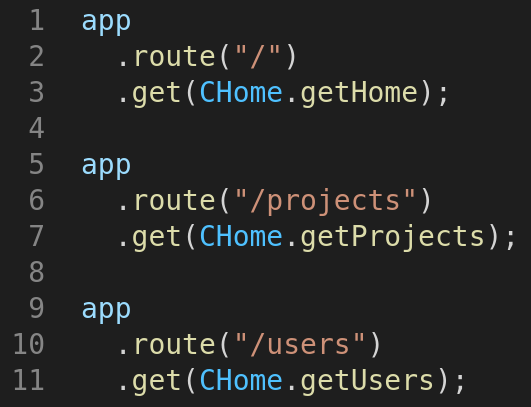
\includegraphics[width=.6\textwidth]{Folders-Files/routes/routes-home.png}
	\centering
	\caption{ساختار فایل home}
	\label{fig:file:routes:home}
\end{figure}
\paragraph{\lr{CHome}:}
شئ حاوی اطلاعات فایل home در پوشه کنترل‌گر است.

\subsection{فایل auth}
در این فایل به مسیرهای احرازهویت شامل ورود، ثبت‌نام و خروج کاربر پرداخته شده است.
\begin{figure}[H]
	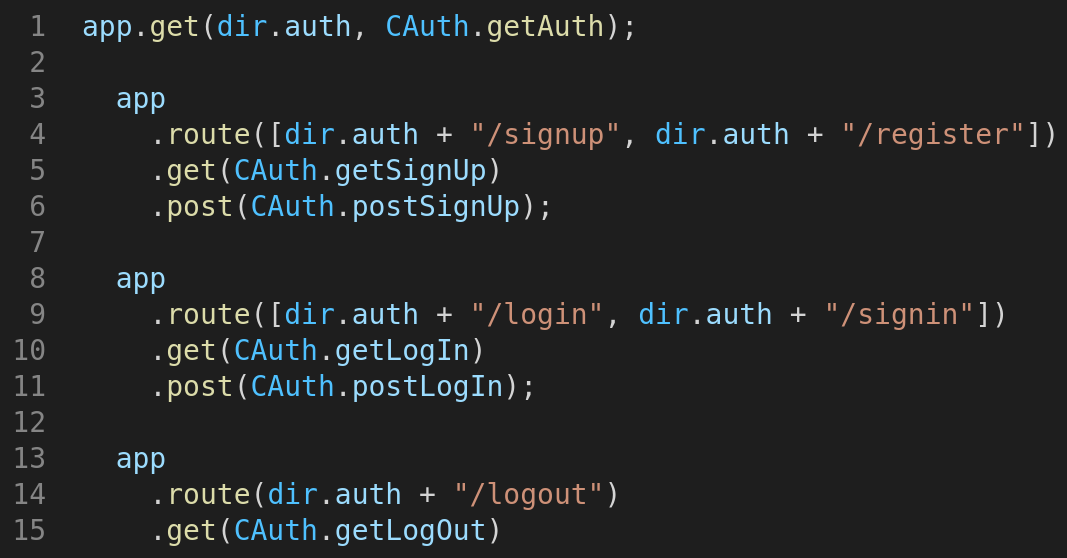
\includegraphics[width=.6\textwidth]{Folders-Files/routes/routes-auth.png}
	\centering
	\caption{ساختار فایل auth}
	\label{fig:file:routes:auth}
\end{figure}
\paragraph{\lr{CAuth}:}
شئ حاوی اطلاعات فایل auth در پوشه کنترل‌گر است.

\subsection{فایل dashboard}
در این فایل به مسیرهای داشبورد کاربر پرداخته شده است.
\begin{figure}[H]
	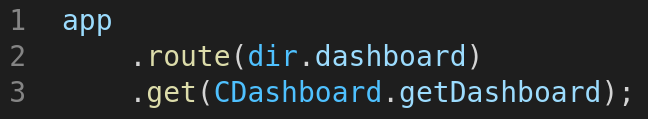
\includegraphics[width=.6\textwidth]{Folders-Files/routes/routes-dashboard.png}
	\centering
	\caption{ساختار فایل dashboard}
	\label{fig:file:routes:dashboard}
\end{figure}
\paragraph{\lr{CDashboard}:}
شئ حاوی اطلاعات فایل dashboard در پوشه کنترل‌گر است.

\subsection{فایل employer}
در این فایل به مسیرهای داشبورد کارفرما پرداخته شده است.
\begin{figure}[H]
	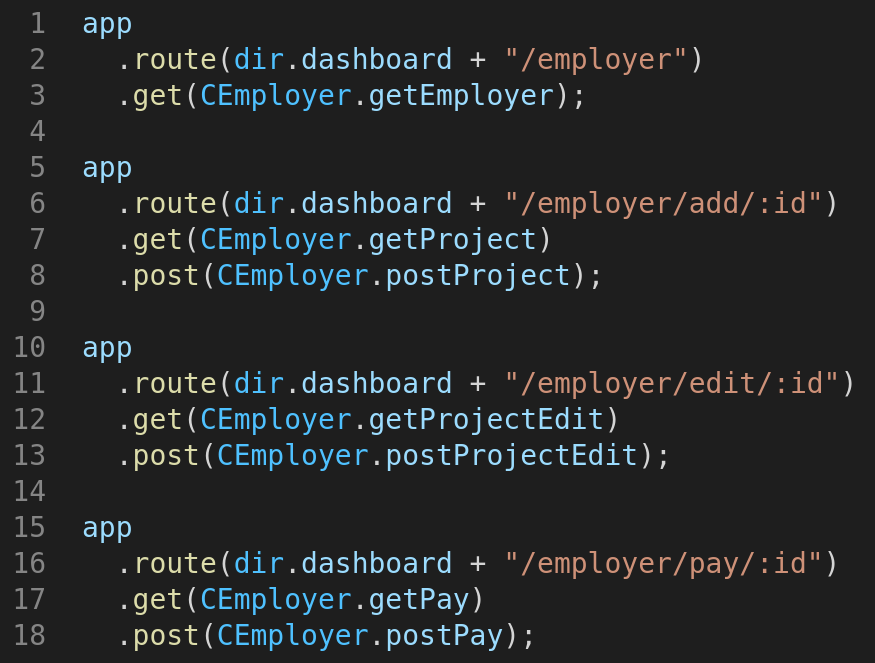
\includegraphics[width=.6\textwidth]{Folders-Files/routes/routes-employer.png}
	\centering
	\caption{ساختار فایل employer}
	\label{fig:file:routes:employer}
\end{figure}
\paragraph{\lr{CEmployer}:}
شئ حاوی اطلاعات فایل employer در پوشه کنترل‌گر است.

\subsection{فایل frelanser}
در این فایل به مسیرهای داشبورد فریلنسر پرداخته شده است.
\begin{figure}[H]
	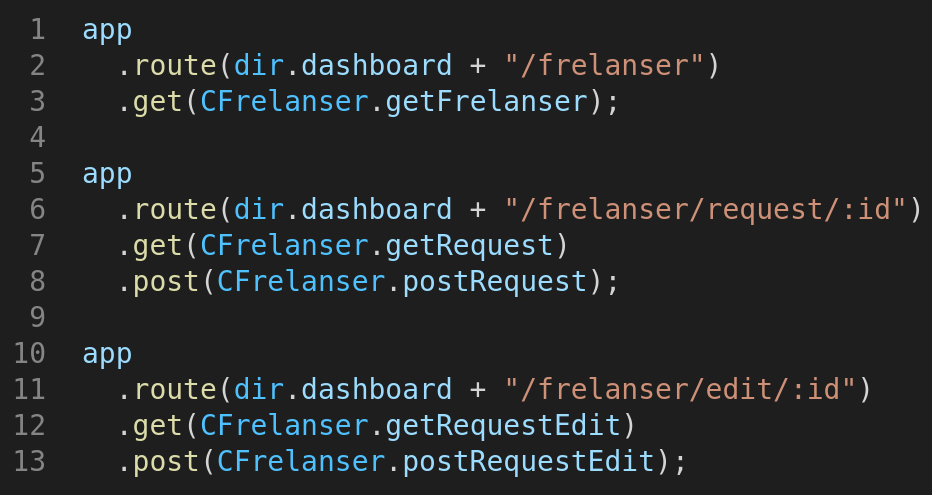
\includegraphics[width=.6\textwidth]{Folders-Files/routes/routes-frelanser.png}
	\centering
	\caption{ساختار فایل frelanser}
	\label{fig:file:routes:frelanser}
\end{figure}
\paragraph{\lr{CFrelanser}:}
شئ حاوی اطلاعات فایل frelanser در پوشه کنترل‌گر است.

